\chapter{Related Work}
\label{chapter:Related_Work}

\begin{figure}[h!]
  \caption{A picture of a gull.}
  \centering
    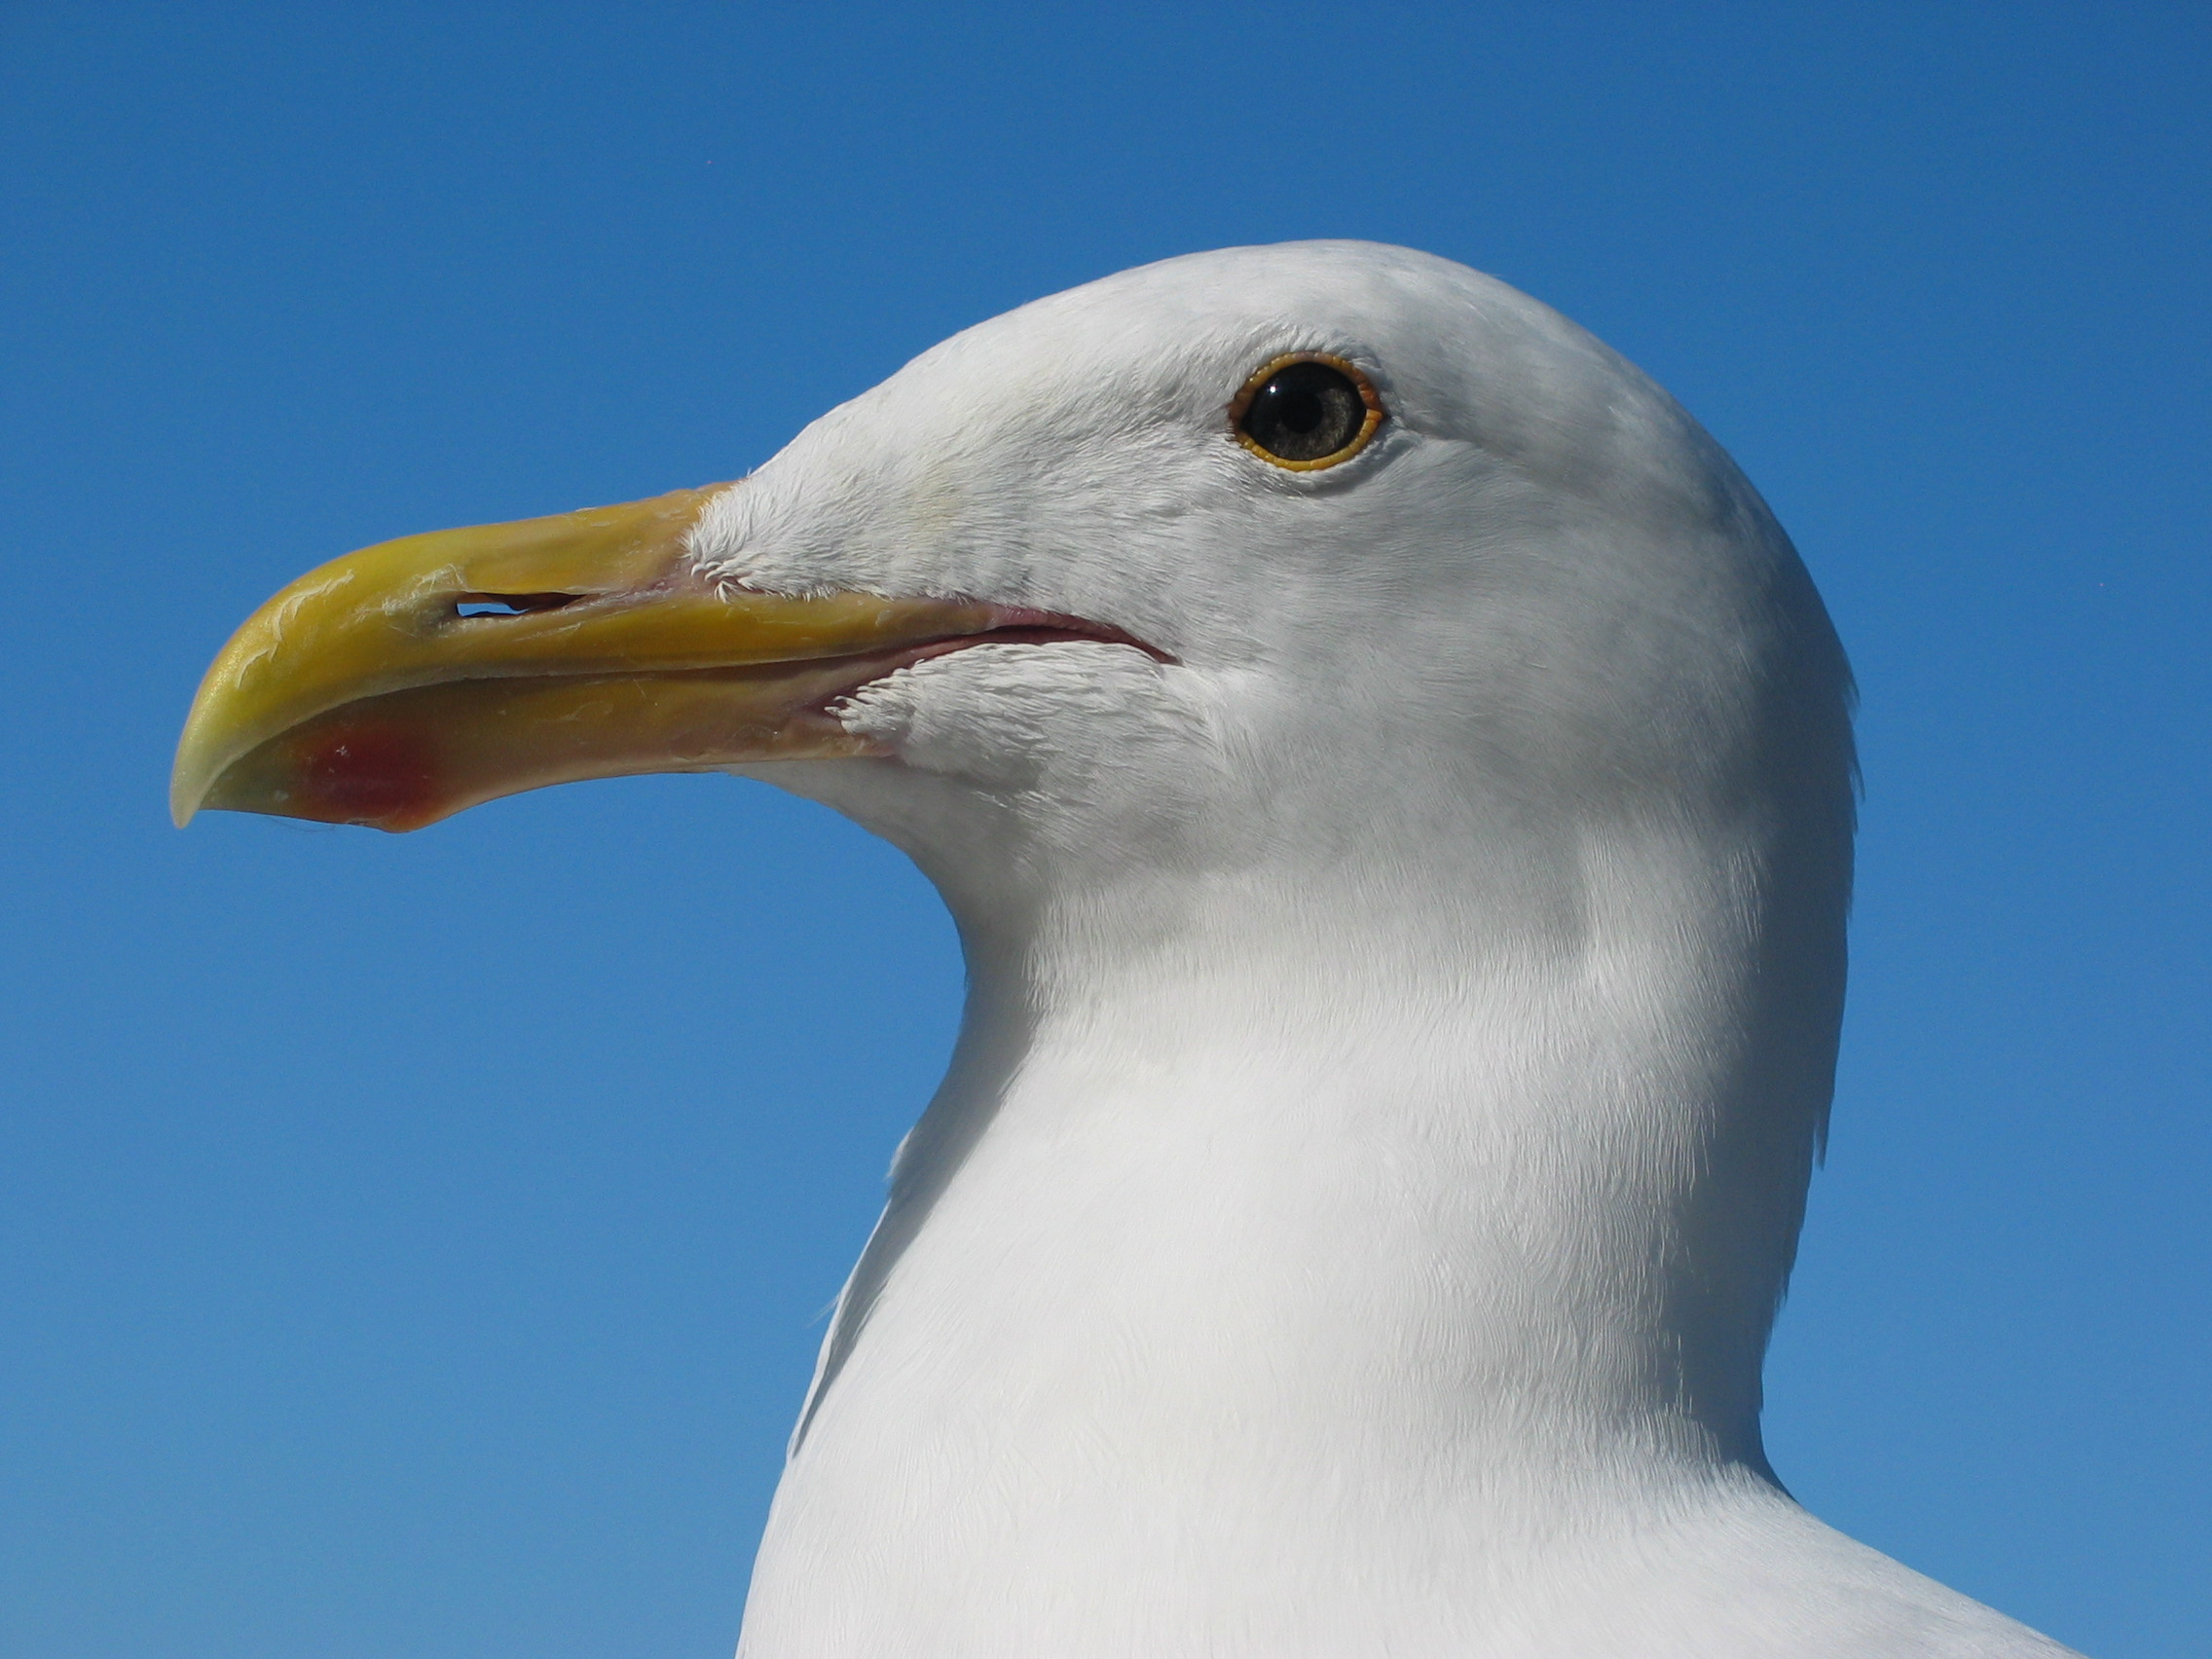
\includegraphics[width=0.8\textwidth]{chapters/images/gull}
\end{figure}

\section{3D geometry}

Yes  - do coordinate systems, transformations, notation
Brief description of SE(3) and SO(3)

\section{Camera Models}

In order to utilise a camera as a sensor, a mapping between camera coordinates and world coordinates
needs to be derived.  To achieve this mapping a model of the camera is required.  This section will
cover all the different types of cameras used in this work and corresponding camera models for
each. 

\subsection{Pinhole Camera Model}

\begin{figure}[h!]
  \caption{Pinhole Camera}
  \centering
    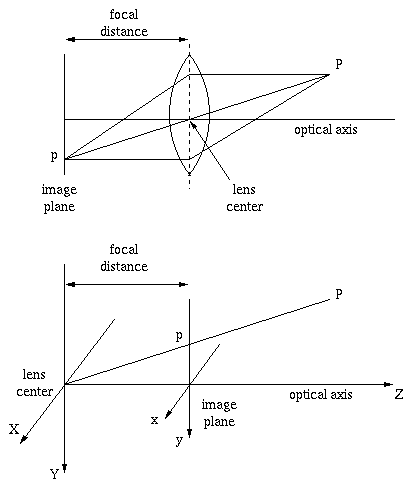
\includegraphics[width=0.5\textwidth]{chapters/images/pinhole_camera}
\end{figure}

\subsection{Stereo Camera}

\subsection{Omni-directional Camera}

\subsection{Flir}
Leave this to last.  Flir may (probably) get left out

\section{Computer Vision Basics}

\subsection{Feature point detection and extraction}

Outline what is feature point detection, description and matching, why we need it.  Mention SIFT
and SURF and cite them.  Mention that we used a GPU implemtation of SIFT, cite the ETH paper. 
Mention a bunch of other descriptors, cite them as well.

\subsection{RANSAC}

explain this cos its easy and fun.  Cite a paper

\subsection{Geometry estimation}

\subsubsection{5 point algorithm}

ask for matthias for relavent literature

\subsubsection{Point triangulation}

ask for matthias for relavent literature

\subsubsection{Stereo pose estimation}

Umeyama (PCL) \newline 
Horn (UVM)


\section{Place Recognition}

Bag of words

\section{Visual SLAM}

Cover this in abstract terms.  Talk about the theory, not implemtation.  Mention PTAM and cite it.
No g2o here.

\subsection{Keyframe SLAM}

\subsection{Graph SLAM}
